\documentclass{article}
\def\npart {2}
\def\nterm {LMS Summer School}
\def\nyear {2020}
\def\nlecturer {Sophie Morier-Genoud : Sorbonne Universite, Paris}
\def\ncourse {Arithmetic and combinatorics of Conway-Coxeter frieze patterns}

\input{header}

\begin{document}
  \maketitle

\section{Overview}
\subsection{Continued fraction}
Let's take $x \in \R$ and we can say, $a < x < a + 1$ where $a \in \Z$. Now we write, $x = a + \frac{1}{x'}$, $x' > 1$.

\begin{align*}
  x = a + \frac{1}{x'} \\
  &= a + \frac{1}{a' + \frac{1}{x''}}\\
  &\vdots\\
  &= a_1 + \frac{1}{a_2 + \frac{1}{a_3 + \frac{1}{\ddots}}}
\end{align*}
where $a_1 \in \Z$ and $a_i \ge 1$ for $\forall i \ge 2$. \\

\begin{nlemma}
  The sequence of $a_i$'s are finite if and only if $x \in \Q$.
\end{nlemma}
\begin{proof}
  If it's finite, it's obvious that it's rational.\\
  Conversely, this is due to Euclid's algorithm. Take $\frac{p}{q} \in \Q$ and then write,
  \begin{align*}
    p &= a_1q + r_1 && 0 \le r_1 \le q\\
    q &= a_2r_1 + r_2 && 0 \le r_2 \le r_1\\
  \end{align*}
\end{proof}
or we can form them by subtracting instead of adding, these make negative expansion (or Hirzebruch-Sung),
$$ x = a_1 - \frac{1}{a_2 - \frac{1}{a_3 - \frac{1}{\ddots}}} $$

\begin{notation}
 $x = [a_1, a_2, \dots]$ means $x$ is a regular continued fraction and $x = [[a_1, a_2, \dots]]$ means a negative expansion.
\end{notation}

  Let's take $x \notin \Q$ and consider the golden ratio,\\
  $$ \varphi = [1, 1, 1, 1, 1, 1, 1, \dots] $$
  and now $e$, there is some regularity,
  $$ e = [2, 1, 2, 1, 1, 4, 1, 1, 6, 1, 1, 8, 1, \dots] $$
  and now $\pi$, there is no regularity,
  $$ \pi = [3, 7, 15, 1, 292, 1, 1, \dots] $$

Now consider the generalised continued fraction,
$$ \pi = \frac{4}{1 + \frac{1^2}{2 + \frac{3^2}{2 + \frac{5^2}{\ddots}}}} $$
Now consider the negative expansion,
$$ \![2, 2, 2, 2, 2, 2, \dots\!] $$
This is just one. It may be represented with an infinite sequence.\\

Here are some more examples,
\begin{align*}
  \frac{5}{2} &= [2, 2] = \![ 3, 2 \!]\\
  \frac{10}{3} &= [3, 3] = \![ 4, 2, 2 \!]\\
  \frac{14}{5} &= [2, 1, 3, 1] = \![ 3, 5 \!]\\
  \frac{43}{16} &= [2, 1, 2, 5] = \![ 3, 4, 2, 2, 2, 2 \!]
\end{align*}

\begin{remark}
  To make it unique one can always choose an even number for the length of the sequence. For a regular expansion, we can always assume that it's of even length.
\end{remark}

There is a very natural question, given $x = [a_1, \dots, a_{2m}] = \![c_1, c_2, \dots c_k \!]$, what is the relationship between $a_i$'s and $c_i$'s?

\subsection{Friezes}
Friezes are from Coxeter in the 1970's. We have the first and last row as 1's. When you have a diamond of numbers,

\begin{figure}[!ht]
  \centering
  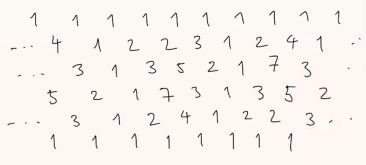
\includegraphics{./figures/L1.1}
  \caption{A frieze pattern}
  \label{}
\end{figure}
%     b
%  a    d
%     c
% ad - bc = 1

\begin{nthm}[Coxeter]
  Friezes are periodic!
\end{nthm}

We shall consider the width of the frieze, don't count the ones. The example has width of 4 and we can look at the width + 4, we get some perdiodic notion. This means we just need the first `row' to fill the frieze.\\

Furthermore, we now have some sort of glide symmetry. We can form triangles and they repeat themselves. Let's finish the statement

\begin{nthm}[Coxeter]
  Friezes are periodic!
  \begin{itemize}
    \item Width $w \to (w+3)$ is a period.
    \item Invariant under a glide symmetry.
  \end{itemize}
\end{nthm}

\begin{ex}
  Exerises 1,2,3 and 4.
\end{ex}

\textbf{Question 2:} How to get frieze containing only positive integers?\\

\subsection{Triangulation of n-gons}

\begin{ndefi}[Diagonal]
  A line that joins two non-consecutive vertices.
\end{ndefi}

\begin{ndefi}[Triangulation]
  The maximum number of non-intersecting diagonals.
\end{ndefi}
The triangulation is not unique. The number of triangulations is related to the Catalan numbers. For every triangulation, you may two or more triangles on the exterior. We will consider exactly two exterior triangles for the minute,\\
Fix a triangulation with two exterior triangles, if you join two external vertices of these external triangles, then you will intersect every other triangle.\\

If you consider the triangles layed next to eachother like this,
\begin{figure}[!ht]
  \centering
  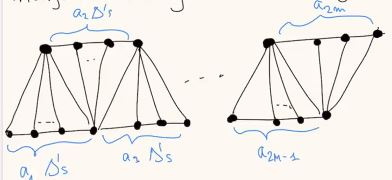
\includegraphics{./figures/L1.2}
  \caption{}
  \label{}
\end{figure}
We can count how many triangles are incidence to the vertex. We shall call this $c_i$ where $i$ is the number of the vertex. If we do this for the 7-gon,
\begin{figure}[!ht]
  \centering
  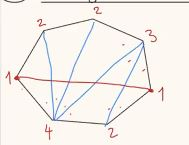
\includegraphics{./figures/L1.3}
  \caption{}
  \label{}
\end{figure}
The sequence $(a_1, a_2, \dots, a_{2n})$ determines the triangulation and the so does the sequence, $(c_1, c_2, \dots)$.

\begin{nthm}
  With this data, we can say that,
  \begin{itemize}
    \item $[a_1, a_2, \dots, a_{2m}] = \![ c_1, c_2, \dots, c_k \!]$
    \item $(c_1, c_2, \dots, c_n)$ determines a frieze of width $n-3$ containing only positive integers.
  \end{itemize}
\end{nthm}

\begin{remark}
  On 1) this is called this Hirzebruch Formula,
  $$ [a_1, a_2, a_3, \dots, a_{2m}] = \![ a_1+1, 2, 2, \dots, 2, a_3+2, 2, \dots \!] $$
\end{remark}

\begin{remark}
  On 2) It works with any kind of triangulations and all friezes arise this way. (This is Conway-Coxeter Theorem) and a Conway-Coxeter Frieze is a frieze with positive integers.
\end{remark}

\end{document}
